\documentclass{report}
\usepackage[utf8]{inputenc}
\usepackage{tocloft}
\usepackage[italian]{babel}

\usepackage{setspace}
\usepackage{graphicx}
\usepackage{geometry}
\usepackage{wrapfig}

\usepackage{listings}
\usepackage{subcaption}
\usepackage{float}
\usepackage{caption}
\usepackage{enumerate}
\usepackage{setspace}
\usepackage{url}
\usepackage{amsmath}

\setcounter{secnumdepth}{6}

\def\code#1{\texttt{#1}}


% Indice e citazioni linkate
\usepackage{hyperref}
\hypersetup{
    colorlinks,
    citecolor=black,
    filecolor=black,
    linkcolor=black,
    urlcolor=black
}


\title{Documento dei Requisiti}
\author{Mattia Busnelli e Salanti Michele}

\begin{document}

\begin{titlepage}
\begin{onehalfspace}
	\begin{wrapfigure}[4]{l}[22mm]{0.25\textwidth}
		\vspace*{-7mm}
		\centering
		
\includegraphics[width=0.25\textwidth]{img/logo_unimib.pdf}
	\end{wrapfigure}
	\par
	\noindent Università degli Studi di Milano Bicocca \\
	\textbf{Scuola di Scienze \\
			Dipartimento di Informatica, Sistemistica e Comunicazione \\
			Corso di Laurea Magistrale in Informatica}
\end{onehalfspace}

\vfill
\par

\begin{doublespace}
\begin{center}
	{\Huge \textbf{\\Sistemi e Servizi di Telecomunicazione}}
\end{center}
\begin{center}
	{\Large \textbf{\\Prestazioni dei firewall realizzati con appliance dedicate: Dipendenza dal numero di regole e ottimizzazioni}}
\end{center}
\end{doublespace}

\vfill
\par

\begin{onehalfspace}

\vspace{8mm}
\par

\begin{flushright}
	{\large \textbf{Autore:} \\
			\textit{Michele Salanti 793091}
	}
\end{flushright}
\end{onehalfspace}

\vfill
\par

\begin{center}
	{\large \textbf{Anno Accademico 2019--2020}}
\end{center}

\end{titlepage}


\renewcommand{\cftsecleader}{\cftdotfill{\cftdotsep}}
\tableofcontents


\chapter{Introduzione}
L'attuale infrastruttura di rete si è stabilizzata per oltre un decennio e si è radicata profondamente nel contesto della società umana. Tuttavia, le imprese ed i fornitori di servizi stanno iniziando a realizzare i forti limiti e l'inflessibilità dello stato attuale dell'infrastrutura con le tecnologie di rete in rapida evoluzione e le crescenti richieste da parte degli utenti.

In altre parole si è riconosciuta la necessità di ristrutturare l'attuale architettura con qualcosa di più dinamico e flessibile \cite{suh2014building}.

\section{Software-Defined Network}\label{sdn}
Come risultato, per superare queste limitazioni intorno al 2005 è stata proposta la \textit{Software-Defined Network} (SDN). SDN è un concetto di rete che sta acquistando tendenza negli ultimi anni, il quale \textit{disaccoppia} il \textit{piano di controllo} e il \textit{piano dati}, \textit{centralizzando} così l'intelligenza di rete in un \textit{controller}.

L'idea di separare il controllo e il piano dati è nata principalmente con l'intenzione di permettere di sviluppare ciascuna parte in modo completamente indipendente l'una dall'altra, in modo che il software non sia vincolato dalla limitazione dell'hardware. Ed eventuali amministratori di rete possano orchestrare la rete per mezzo di applicazioni di alto livello, semplificandone la gestione \cite{fundation2012software}\cite{suh2014building}.

In altre parole si abbandona completamente la concezione verticale e monolitica di apparati di rete "tutto-in-uno", con l'intero stack (sia hardware e software) fornito da un'unica compagnia.
\newline
\newline
In caso di cambiamenti alla rete, anziché dover configurare manualmente ogni singolo switch in conformità di questi cambiamenti, è possibile utilizzare switch programmabili controllati da un'unica applicazione esterna.

\section{OpenFlow}\label{openflow}
Il componente più importante della SDN è un protocollo di comunicazione \textit{tra il piano di controllo ed il piano dati}. Il \textit{\textbf{protocollo OpenFlow}} è stato introdotto a tale scopo, supportato dalla \textit{Open Networking Foundation} (ONF); allo stato attuale, sono disponibili controller SDN open source che implementano OpenFlow, i più noti sono: \textit{NOX}, \textit{POX}, \textit{Ryu} e \textit{Floodlight} \cite{suh2014building}.

\section{Obiettivo}
Vista la nativa caratteristica delle SDN di effettuare azioni sul flusso del traffico, in particolare azioni come \textit{scartare} pacchetti (drop) o \textit{permetterne il passaggio} ed il diffuso utilizzo del protocollo OpenFlow, in questa relazione andremo a vedere alcune funzioni di firewall implementate tramite questa relativamente \textit{"nuova"} (2005!) architettura e protocollo ed ai possibili vantaggi e risvolte che è possibile avere sia nella sicurezza che nella gestione di reti.


\begin{figure}[H]
  \centering
    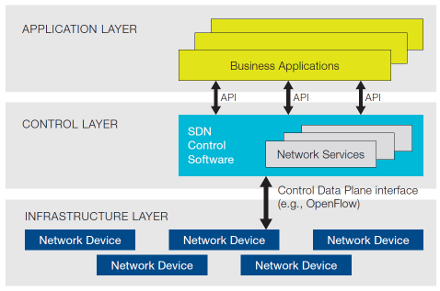
\includegraphics[width=\linewidth]{img/sdn-arch.png}
    \caption{Paradigma SDN}
  \label{fig:coffee}
\end{figure}


\chapter{Contesto Applicativo e Motivazioni}
\onehalfspacing
\section{Contesto Applicativo}

\subsection{Firewall}\label{firewall_cont}
Un \textit{\textbf{firewall}} è un componente \textit{software}, \textit{hardware} o una \textit{combinazione dei due} che filtra i flussi di traffico di rete, solitamente posto ai confini di essa. Filtra il traffico consultando una \textit{tabella di regole definite staticamente} che definiscono quale traffico può o non può passarci attraverso.
\newline
Le regole sono tradizionalmente espresse in \textit{cinque} tuple: 

\begin{itemize}
  \item indirizzo IP di origine
  \item indirizzo di destinazione
  \item protocollo di trasporto
  \item numero della porta di origine
  \item numero della porta di destinazione
\end{itemize}

I firewall possono utilizzare \textit{due} metodi di filtro contrastanti per applicare una politica di sicurezza della rete. Questi metodi possono essere descritti come \textit{permissivi} o \textit{restrittivi} \cite{collings2014openflow}.

I \textbf{\textit{firewall permissivi}} non eliminano il traffico per impostazione predefinita, a meno che non sia specificato. Al contrario, i \textbf{\textit{firewall restrittivi}} eliminano tutto il traffico per impostazione predefinita. In entrambi i casi, i flussi desiderabili di traffico richiedono precise specifiche, rispettivamente tramite \textit{blacklist} e \textit{whitelist}.

\subsection{Lavori collegati}\label{works}
I firewall basati su OpenFlow sono stati sviluppati e studiati nella ricerca per vari scopi.

Il lavoro del gruppo di \textit{Suh} \cite{suh2014building} per esempio si concentra sul miglioramento dell'interfaccia uomo-firewall per facilitare agli amministratori di rete l'installazione e l'aggiornamento delle politiche di rete, mentre il gruppo di \textit{Collings} \cite{collings2014openflow} sviluppa un firewall al fine di presentare un quadro di valutazione delle prestazioni di base per misurare l'overhead di comunicazione tra il controller e lo switch.

\textit{Wang} \cite{wang2013towards} si concentra sulle possibili problematiche e sfide per quanto concerne la sicurezza ed implementare firewall robusti basati su SDN.

Infine \textit{Bakker} \cite{bakker2016network} cerca di sfruttare appieno le capacità del paradigma SDN con OpenFlow e di spostare il concetto di firewall da elemento visto come barriera/filtro posto ai confini della rete ad elemento esteso su tutta la rete composto da una od una serie di poliche a seconda del tratto di rete che si va a considerare.

Quest'ultimo lavoro è quello su cui l'autore di questo scritto ha deciso di \textit{focalizzare l'attenzione}.


\section{Motivazioni}

I firewall tradizionali si limitano a filtrare il traffico nei loro punti di distribuzione.
Le ricerche sinteticamente presentate nel paragrafo \ref{works} hanno dimostrato che OpenFlow è una tecnologia adatta per il filtraggio dei pacchetti in una rete, tuttavia, eccetto per il lavoro del gruppo di \textit{Bekker} \cite{bakker2016network} non sembra essersi prestata sufficiente attenzione al modo in cui può essere utilizzata per filtrare in modo flessibile il traffico attraverso una rete che implementa di più di uno switch.

Un altro motivo per cui questo argomento merita più attenzione è che è potenzialmente una \textit{valida alternativa} al dover comprare (e poi integrare e mantenere) costosi firewall esterni dedicati da fornitori come Cisco o Juniper, ognuno con il proprio stack dedicato \cite{suh2014building}; che per giunta non è detto che siano facilmente integrabili tra di loro (tra marche diverse), oltre che mantenibili e scalabili se si guarda anche con un'ottica a lungo termine.

\subsection{Firewall non solo ai confini della rete}\label{firewall_confini}
Quello che il gruppo di \textit{Bekker} propone è un firewall virtuale basato su OpenFlow in grado di filtrare il traffico di rete attraverso \textit{un'intera rete, non solo ai limiti} \cite{bakker2016network}. Di conseguenza, i dispositivi di rete possono essere protetti indipendentemente dalla loro posizione e il firewall non può essere più un singolo punto di vulnerabilità (SPOF).

La soluzione proposta offre flessibilità grazie alla possibilità di raggruppare le regole del firewall in domini di politiche (policy domains) che possono quindi essere assegnati agli switch OpenFlow; l'applicazione delle regole può essere selettiva in base a criteri diversi ed arbitrari come posizione, ora, tipo di dispositivo, ecc...

\subsection{Nella pratica}
In pratica se ogni switch ethernet potesse funzionare come un firewall tradizionale, cambierebbe il modo in cui la politica di sicurezza viene implementata in un ambiente di rete. Immaginiamo se ogni switch ethernet fosse un firewall multiporta, quindi i criteri del firewall potrebbero essere implementati in tutta la rete, su ogni porta di ingresso di switch e su ogni collegamento tra switch. Ci sarebbero firewall per ogni server, desktop, ed ogni altro collegamento e la politica del firewall sarebbe implementata da un \textit{controller} che mantiene una visione \textit{\textbf{globale}} del traffico dell'applicazione corrente e potere decisionale su quale traffico dovrebbe essere consentito.

Avere una o più politiche di sicurezza applicata su tutto l'ambiente significherebbe una vera e propria \textit{\textbf{erosione del perimetro}} \cite{opengroup_erosion} di sicurezza della rete stessa.

Questo andrebbe tamponare in maniera non trascurabile il problema nella sicurezza che pone la politica negli ultimi anni di permettere agli utenti di collegare alla rete interna dell'organizzazione i propri dispositivi personali invalidando automaticamente l'oramai obsoleto \textit{"assioma"} che il traffico malevolo può venire solo dall'esterno \cite{bakker2016network}.

Detto questo, avere molte politiche di sicurezza implementate da gestire manualmente sarebbe un vero inconveniente. Tuttavia, come accennato nei paragrafi \ref{sdn} e \ref{openflow} con un'architettura di controller, la politica (policy) verrebbe creata una volta sola e poi trasferita atuomaticamente a tutti i dispositivi di rete associati per essere applicata.


\chapter{Implementazione}
\onehalfspacing

\section{Struttura}


Il firewall controller può potenzialmente essere posizionato in un qualsiasi punto della rete. Le regole sono specificate nella tabella di flusso che sono gestite sia dallo switch che dal firewall controller (vedi tabella \ref{fig:flow}). Una voce nella tabella di flusso corrisponde ad una regola che gestisce il flusso del traffico. Lo switch agisce come un banale inoltratore di pacchetti basato sulle regole di sicurezza definite nella sua tabella di flusso. Il firewall controller utilizza la sua tabella di flusso per tenere traccia delle decisioni intraprese sul traffico.

Un canale di comunicazione dedicato viene mantenuto tra lo switch e il controller del firewall. Attraverso questo canale, lo switch invia le informazioni sui flussi di traffico non identificati al controller per l'ispezione e il controller invia le decisioni allo switch.

\begin{figure}[H]
  \centering
    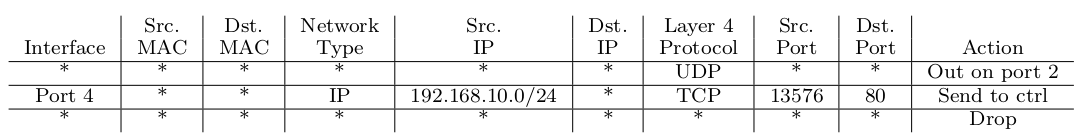
\includegraphics[width=\linewidth]{img/flow.png}
    \caption{Esempio di Tabella di Flusso (Flow Table)}
  \label{fig:flow}
\end{figure}

\section{Modalità Permissiva e Restrittiva}

Sono state presenti due modalità per specificare le azioni di controllo predefinite in base al traffico:

\begin{itemize}
  \item \textbf{\textit{Modalità permissiva:}} rifiuto selettivo dei flussi. Ossia che il traffico viene normalmente inoltrato di default a meno che non venga esplicitamente negato.
  \item \textbf{\textit{Modalità restrittiva:}} autorizzazione selettiva dei flussi. Ossia che il traffico viene negato di default a meno che esplicitamente consentito.
\end{itemize}


\section{First Deny Last Allow}
Un controller firewall adotta una metodologia \textit{"first deny last allow"} per determinare un'azione di controllo su un flusso.

Un controller privilegia flusso che "matcha" (corrisponde) ad una regola di rifiuto (deny rule) rispetto a una regola di permissiva (allow rule). La precedenza delle regole di rifiuto sulle regole di consenso allevia il rischio per la sicurezza derivante da regole potenzialmente in conflitto nella tabella di flusso del controller ed anche evita che i pacchetti debbano percorrere un'intero set di regole prima di essere scartati.


\section{Posizione delle regole: Valutazione delle performances}

In seguito verranno brevemente presentate le prestazioni di un firewall di rete basato su regole. In genere, e come mostrato nella Figura \ref{fig:firewallrulebase}1, i pacchetti in entrata che trasportano richieste arrivano al firewall e vengono messi in coda per l'elaborazione in più fasi:

\begin{enumerate}
  \item La prima fase prevede l'esecuzione di funzionalità di collegamento dati e livello di rete.
  \item Successivamente viene attivato il motore di ricerca delle regole del firewall per elaborare i pacchetti in entrata.
\end{enumerate}

Salah cita da un'altra fonte \cite{salah2011performance} che è stato dimostrato che le regole in fondo alla tabella possono essere scoperte da un aggressore esterno. Un utente malintenzionato può quindi lanciare un attacco che prenda di mira principalmente le regole di in fondo alla tabella e degradi efficacemente e rapidamente le prestazioni di un firewall con una serie di attacchi DoS a basso volume di traffico. Questo tipo di attacco viene chiamato "attacco di complessità algoritmica" (Complexity-algorithmic attacks), è una classe di attacchi DoS a bassa velocità che sfruttano le carenze algoritmiche nella progettazione del software \cite{salah2011performance}.

Risulta quindi importante capire che impatto possono avere questi attacchi sulle prestazioni dei firewall in modo da trovare modi per mitigare il problema.

\subsection{Misure prese}

Il tema di Salah ha effettuato le misurazioni sottoponendo il firewall a due tipi di traffico: traffico normale e traffico DDoS indirizzato a regole diverse situate in posizioni diverse nell'insieme di regole del firewall.
\newline
\newline
In base all'hardware a disposizione del team è stato misurato che:
\begin{itemize}
  \item Il valore medio era di circa 0,5 ms per l'interrogazione di 10.000 regole, ossia 0,05 microsecondi per singola regola.
  \item Il tempo medio di elaborazione del kernel del driver del dispositivo e dell'elaborazione IP ed è stato riscontrato che il valore medio è di circa 2,65 microsecondi.
\end{itemize}

\begin{figure}[H]
  \centering
    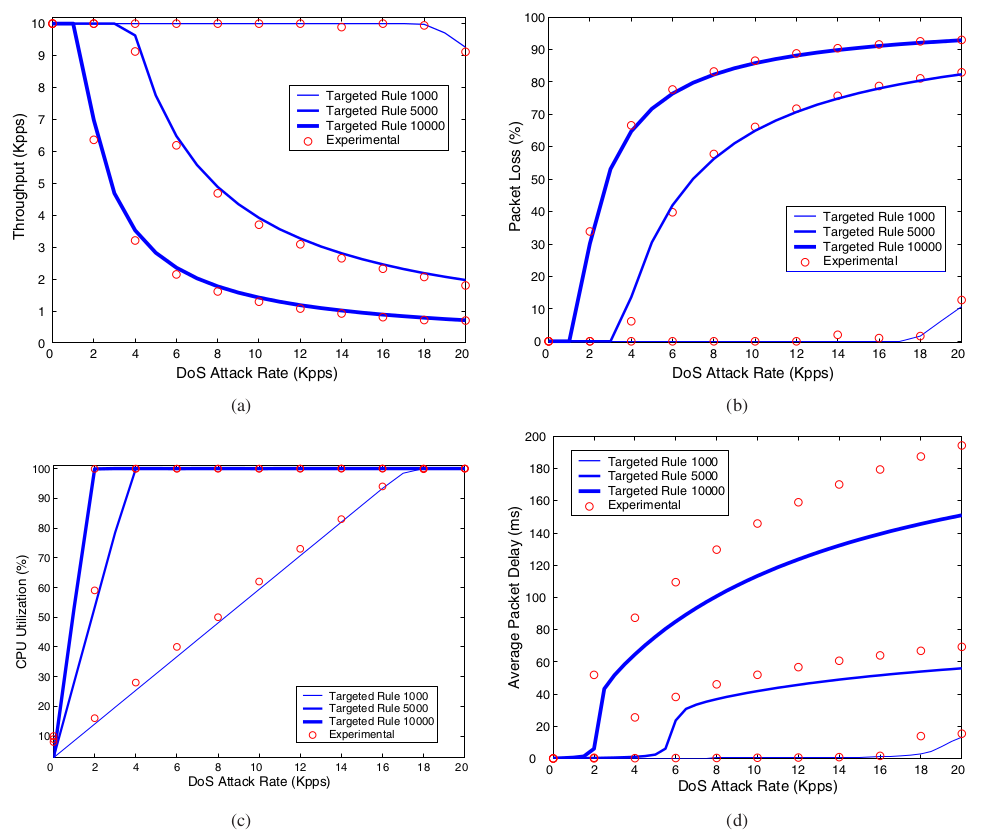
\includegraphics[width=\linewidth]{img/dos.png}
    \caption{L'impatto dei flussi di traffico DoS che colpiscono diverse regole sul firewall}
  \label{fig:dos}
\end{figure}

La Figura \ref{fig:dos} mostra l'impatto sulle prestazioni che il firewall subisce quando si lanciano attacchi DoS con velocità diverse che colpiscono posizioni diverse delle regole. L'impatto è stato misurato facendo in modo che venga generato un normale flusso di traffico UDP costante a una velocità di 10 Kpps.

Abbiamo misurato il degrado delle prestazioni in termini di perdita di pacchetti (packet loss), velocità effettiva, utilizzo della CPU e ritardo unidirezionale quando si invia traffico normale e quando si sottopone il firewall a flussi di attacchi DoS di velocità diverse e prendendo di mira regole diverse.

\subsection{Osservazioni}

Dai grafici mostrati in Figura \ref{fig:dos} emerge chiaramente che un leggero degrado si manifesta quando gli attacchi DoS prendono di mira le regole più importanti (quelle in cima), mentre un notevole degrado si manifesta quando gli attacchi DoS colpiscono regole meno importanti (quelle in fondo) come quelle posizionate a 5.000 e 10.000. Più specificamente, quando si prendono di mira le regole meno importanti, si può osservare un degrado grave e evidente con attacchi DoS a velocità relativamente bassa di circa 1 Kpp e 3 Kpp quando si prendono di mira regole posizionate rispettivamente a 10.000 e 5.000. Tuttavia, quando si prende di mira una regola posizionata a 1000, il degrado si manifesta solo con attacchi DoS ad alta velocità di circa 18 Kpps.

Pertanto, si può concludere che le regole di targeting nella parte inferiore del set di regole possono essere gravemente dannose per le prestazioni del firewall. Le prestazioni del firewall sono accettabili quando gli attacchi DoS (fino a una velocità di 18 Kpps) mirano a regole posizionate intorno a 1.000, ma non a regole superiori.

\section{Conotroller: Valutazione delle performances}

Nella valutazione, il team di Collins fa uso di una configurazione restrittiva con insiemi di regole composte completamente da regole permissive (allow rules). Ciò rappresenta il caso di regole base peggiore perché il controller del firewall è costretto a tentare di accettare ogni flusso di traffico non identificato.

Il numero di regole nelle configurazioni varia da un minimo di 3 a un massimo di 1000.

\begin{figure}[H]
  \centering
  \begin{subfigure}[b]{0.46\linewidth}
    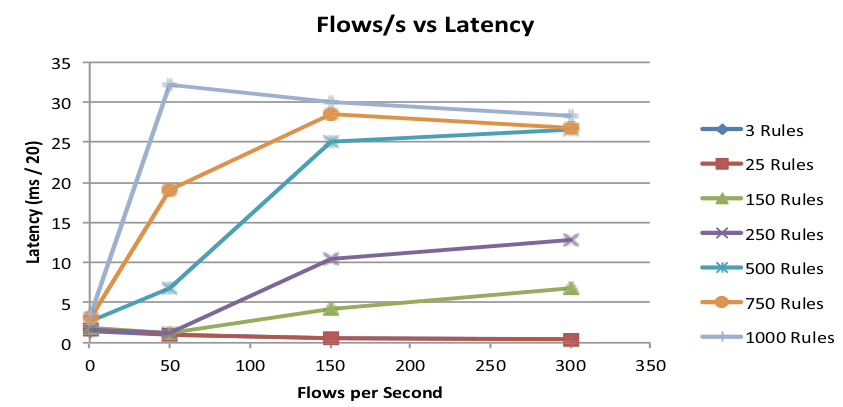
\includegraphics[width=\linewidth]{img/flow_latency.png}
    \caption{Crescita della latenza media}
    \label{fig:flowlatency}
  \end{subfigure}
  \begin{subfigure}[b]{0.46\linewidth}
    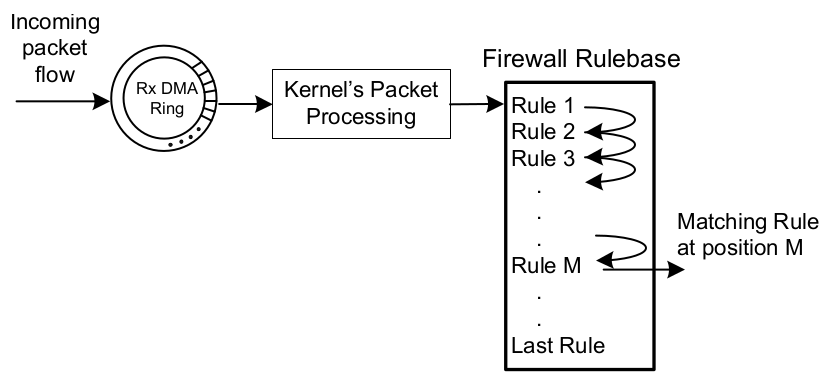
\includegraphics[width=\linewidth]{img/firewall_rulebase.png}
    \caption{Schema di interrogazione delle regole del firewall per i pacchetti in arrivo}
    \label{fig:firewallrulebase}
  \end{subfigure}
\end{figure}

Dal grafico \ref{fig:flowlatency} si osserva che la latenza media aumenta linearmente con il tasso di arrivo di nuovi flussi di traffico quando la dimensione del set di regole è 150. Le latenze medie mostrano improvvisi aumenti di latenza con un numero più alto di arrivi di flussi quando le dimensioni del set di regole è a 250 e 500. La latenza media smette di crescere quando il set di regole è a 750 e 1000.

Questa interruzione di crescita, secondo Collins può essere dovuta principalmente a due motivi:

\begin{enumerate}
  \item Molti nuovi flussi di traffico hanno pattern molto simili, quindi dopo un iniziale processamento da parte del controller le regole per quel pattern vengono applicate allo switch. Questa cosa viene osservata spesso in molti flussi di traffico di un gateway principale dove per esempio, molte connessioni Web tentano di visitare lo stesso insieme di server (per esempio portali di News molto frequentati).
  \item Molti flussi vengono scartati (dropped) a causa dello spazio di coda limitato per contenere i pacchetti dei flussi non identificati quando i tassi di arrivo dei flussi sono elevati. La latenza media mostrata in tabella non copre i flussi persi.
\end{enumerate}



\chapter{Note Finali}
\onehalfspacing


Il team di Salah ha dimostrato che le regole di targeting nella parte inferiore (in basso) di un set di regole relativamente ampio possono essere gravemente dannose per le prestazioni di un firewall. Come buona pratica di progettazione e contromisura vitale contro gli attacchi DoS che prendono di mira le regole in fondo al set, il team consiglia di ridurre al minimo le dimensioni del set di regole del firewall o di riorganizzare dinamicamente le regole in modo che le regole più in basso possano essere spostate nella parte superiore del set di regole, rendendolo così più difficile lanciare attacchi algoritmici di tale complessità che colpiscono le regole inferiori.

Il lavoro del team di Collins, a parere dell'autore di questo testo, sembra in parte inconclusivo su questo fronte, ma mostra chiaramente l'impatto della dimensione del set di regole sulle prestazioni d un firewall ed accenna (o da una breve introduzione) a problematiche nuove introdotte dal paradigma SDN che vengono approfondite da ricerche come quella del team di Shin \cite{shin2013fresco} e dal team di Porras \cite{porras2012security} (in breve: Garbage collection delle regole mandate agli switch ed ottimizzazione e risoluzione di conflitti).


Oltretutto, \textbf{\textit{come nota personale}}, l'autore di questo testo si sente di aggiungere che la metodologia \textit{"first deny last allow"} descritta da Collins ed usata anche dal team di Bakker \cite{bakker2016network} può essere una buona tecnica da tenere in mente quando si progettano set di regole di un firequall, indipendentemente che sia SDN-based o meno. Questo, oltre a conferire un ovvio vantaggio sulla mantenibilità da parte degli amministratori di rete, permette anche di garantire prestazioni ottimali dovuto ad un set ridotto di regole.


\bibliographystyle{unsrt}
\bibliography{bibliography.bib}

\end{document}
